\documentclass[10pt,twocolumn,letterpaper]{article}

\usepackage{cvpr}
\usepackage{times}
\usepackage{epsfig}
\usepackage{graphicx}
\usepackage{amsmath}
\usepackage{amssymb}

% point to the figures
\graphicspath{ {images/} }

% Include other packages here, before hyperref.

% If you comment hyperref and then uncomment it, you should delete
% egpaper.aux before re-running latex.  (Or just hit 'q' on the first latex
% run, let it finish, and you should be clear).
\usepackage[breaklinks=true,bookmarks=false]{hyperref}

\cvprfinalcopy % *** Uncomment this line for the final submission

\def\cvprPaperID{****} % *** Enter the CVPR Paper ID here
\def\httilde{\mbox{\tt\raisebox{-.5ex}{\symbol{126}}}}

% Pages are numbered in submission mode, and unnumbered in camera-ready
%\ifcvprfinal\pagestyle{empty}\fi
\setcounter{page}{1}
\begin{document}

%%%%%%%%% TITLE
\title{A Low Cost Eye-tracking Interface to Help the Physically
  Impaired Users}

\author{Thomas Karpati (SCPD)\\
Stanford University \\
{\tt\small tkarpati@stanford.edu}
% For a paper whose authors are all at the same institution,
% omit the following lines up until the closing ``}''.
% Additional authors and addresses can be added with ``\and'',
% just like the second author.
% To save space, use either the email address or home page, not both
\and
Shankar Thadhalani (SCPD)\\
Stanford University \\
{\tt\small shankart@stanford.edu}
}

\maketitle
%\thispagestyle{empty}

%%%%%%%%% ABSTRACT
\begin{abstract}
This paper presents a low cost alternative to traditional
gaze-tracking systems to help pysically impaired uses interact with
machines. We propose a passive system which can utilize the integrated
cameras already present in most laptops and tablets available
today. The system utilizes face and eye tracking to locate the user in
the camera frame and a convolutional neural network to infer the
point-of-gaze of the user from the captured image from the integrated
camera. Due to the passive nature of our system, it doesn't require
the expensive active external lighting sources required by most
existing solutions. The system also doesn't require the user to remain
in a fixed position or to immobilize their head to use the system.
\end{abstract}

%%%%%%%%% BODY TEXT
\section{Introduction}
A gaze-tracking system has numerous application in human computer
interfaces, from use as an input modality for the impaired\cite{calvo}, to
determination of region of interest for augmented reality and image
processing. The goal of gaze-tracking is to determine the location
that a user is looking at. For aiding the impaired, the system would
determine the location on the screen that a user is looking, and then
move the cursor to that location. This can be used as a form of input
for those that cannot move a mouse or use a keyboard. This
can then be used with in on-screen keyboard to interact with a
system.

The system proposed is a completely passive system that uses a single
camera. The system attempts to eliminate the need for expensive
external equipment, just using the integrated camera available on most
laptops and tablets. The system is composed of two main parts. The first
part is to determine the location of the user in the frame of the camera, and the
location of the eyes. To this end, we segment the face of the user
from the rest of the image. Then the left and right eyes are are each
segmented from the face. This information, the location of the face,
the two eyes and the images of the two eyes, is then fed into a
convolutional neural network to determine the point of gaze of the
user from the information determined from the camera image.

Beyond the location of the eye within the eye socket, the system must
also determine the head pose since the user is not required to have
their head constrained or immobilised, and as such the location and
pose of the head is not known a priori. This requires that the
convolutional network must also be passed the location of the eyes in
the frame and the location of the eyes relative to the face to effectively be
able to determine the pose of the users head.


\section{Existing Solutions}
Many existing systems rely on external
devices\cite{eyetrackerlist}\cite{tobii_1}, or require the user to
have their head immobilized or wear a camera attached to their
head. This makes eye tracking an expensive and unreachable solution
for many. Some of these are based on infrared light sources and rely
on the reflection of the light from the user's pupils to identify the
point of user interest. Our system hopes to work around the use of
these external devices. A brief introduction to an existing solution
mechanism can be seen Figure~\ref{fig:existsol}.

\begin{figure}
  \begin{center}
    \includegraphics[width=\linewidth]{existing_solutions}
  \end{center}
  \caption{Existing solutions to gaze-tracking problem}
  \label{fig:existsol}
  \end{figure}

One of the most popular commercials solutions by Tobii Tech consist of varity of 
illuminators, a high resolution NIR sensor, on board embededd core to 
assist image processing and sensor-illumination-synchronization, 
and a high frame rate camera modified for imroved eye tracking. 
The illuminators project a dot matrix on user and NIR sensor along with 
high speed camera take pictures of user's eyes. The inputs from NIR sensor 
and camera are processed to find reflection patterns by on board embedded core, 
which are used to mathematically evaluate points of interest. 
This certainly gives the commercial solution edge over other implementation.

The literature contains systems that are built with strictly classical
approaches to those that are built on more modern neural networks for
processing\cite{krafka}\cite{mcmurrough}\cite{weidenbacher}\cite{baluja}\cite{cazzato}\cite{li}. Our
system hopes to use both methods where we can preprocess the data that
is fed into the network using classical methods to aid in the
processing. We hope to leverage the existing dataset that was produced
by the group at University of Texas, Arlington\cite{mcmurrough}. Their
work contains several videos with synchronized homographies that link
the location and pose of the eyes with the location of the screen
relative to each other. This solution however requires a user to have
a head mounted camera to capture a video of the eyes moving in the
user's eye sockets. While this may be effective, it can be cumbersome
for the user.


\section{Related Work}
Eye tracking has being studied over hundred years, a great deal of
research has gone into studies of the mechanisms and dynamics of eye
rotation, but the goal of eye- tracking is most often to estimate gaze
direction.  The papers which are closely relevant to our work using a
convolutional network are "Eye Tracking for Everyone"\cite{krafka} and "Webcam-Based Eye Movement Analysis Using CNN"\cite{zhaomeng}.

In the paper "Eye Tracking for Everyone", authors implemented a
solution for Apple iOS mobile devices. It used iOS libraries to
identify faces and eyes. The authors used crowd sourcing to collect a large-scale dataset. The training of the system required manual intervention, and user to physically interact with the device. 

In "Webcam-Based Eye Movement Analysis Using CNN", the authors Meng
and Zhao take a different approach at collecting data. They utilized a
widely popular web camera to capture user images for training. Their experiments obtained a large manually sanitized data to test their neural network. 

There are some other non-CNN based experiments based on a paper by Fabian Timm - "Accurate Eye center localization by means of Gradient". 

\section{Technical Approach}
The system was implemented in Python 2.7, using both the OpenCV
libraries and the TensorFlow libraries. The OpenCV libraries provide a
hardware abstraction layer to video capture and display
peripherals. The system was designed to run 2 threads, one thread to
capture and validate input from webcam and another to process the
captured input. The second thread processes the captured and
sanitized input through our convolutional neural network and obtains
the point of user interest on the screen. We merged these 2 threads to
improve reliability, and we faced some lag in response as a compromise. In
following sections, we explain the submodules of the system from image
capturing to evaluating point of interest.

\subsection{Image capture and face/eye detection}
We use haar-cascade utilizing Viola-Jones face recognition algorithm to 
identify face and eyes. First we capture an input stream using the peripheral
interface provided by OpenCV. 

We convert each frame as it is captured to grayscale, this frame is then analyzed 
using Viola-Jone's haar-feature based cascade classifier to identify a face.  
The Viola-Jones algorithm being utilized by the underlying framework is very robust, 
high-speed, and focused on face detection only. This framework doesn't 
identify the individuals. 

A few common properties of human face are used to recognize the face, for example: the human eye region is darker than the upper-cheeks and the nose bridge region is brighter than the eyes. The Viola-Jones object detector classifies images based on such feature values instead of pixels.  A feature based system operates much faster than pixel based systems. Rectangle features are computed integral image. An integral is an intermediate representation for the original image. 
We opted out to use face detection haar-cascade provided by OpenCV, as it is already trained with more than 5000 face images and 300 million non-face images with varying poses, and varying illumination across many individuals. 

\begin{figure}
  \begin{center}
    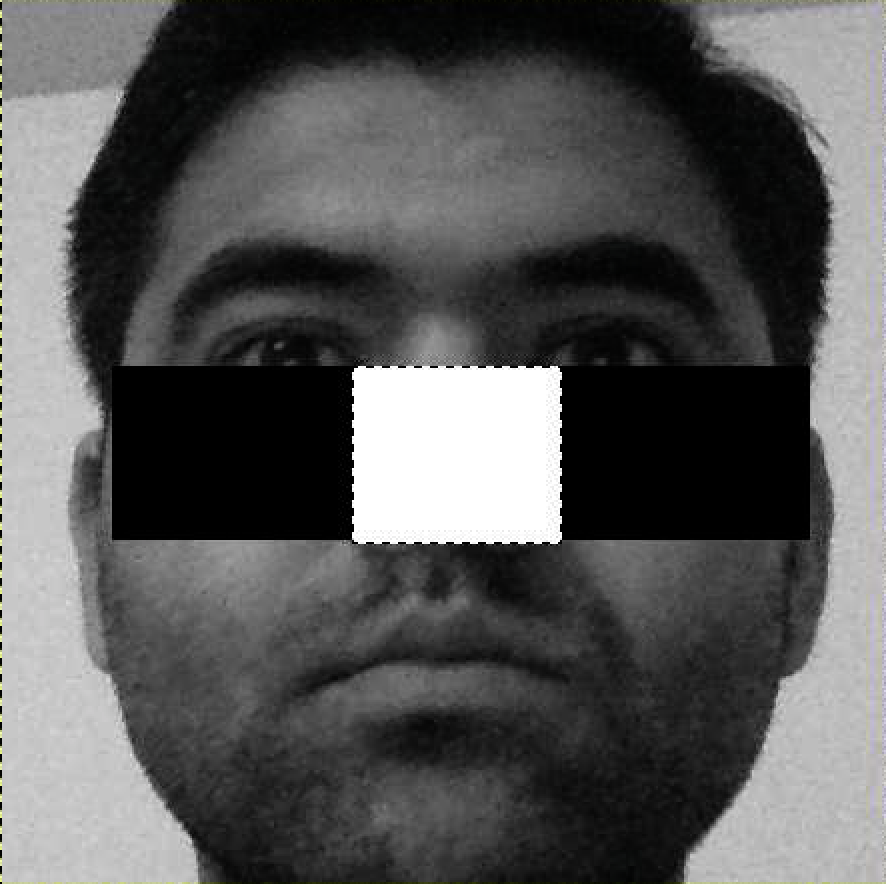
\includegraphics[width=\linewidth]{nose}
  \end{center}
  \caption{Human nose region haar-feature}
  \label{fig:human_nose}
\end{figure}

\begin{figure}
  \begin{center}
    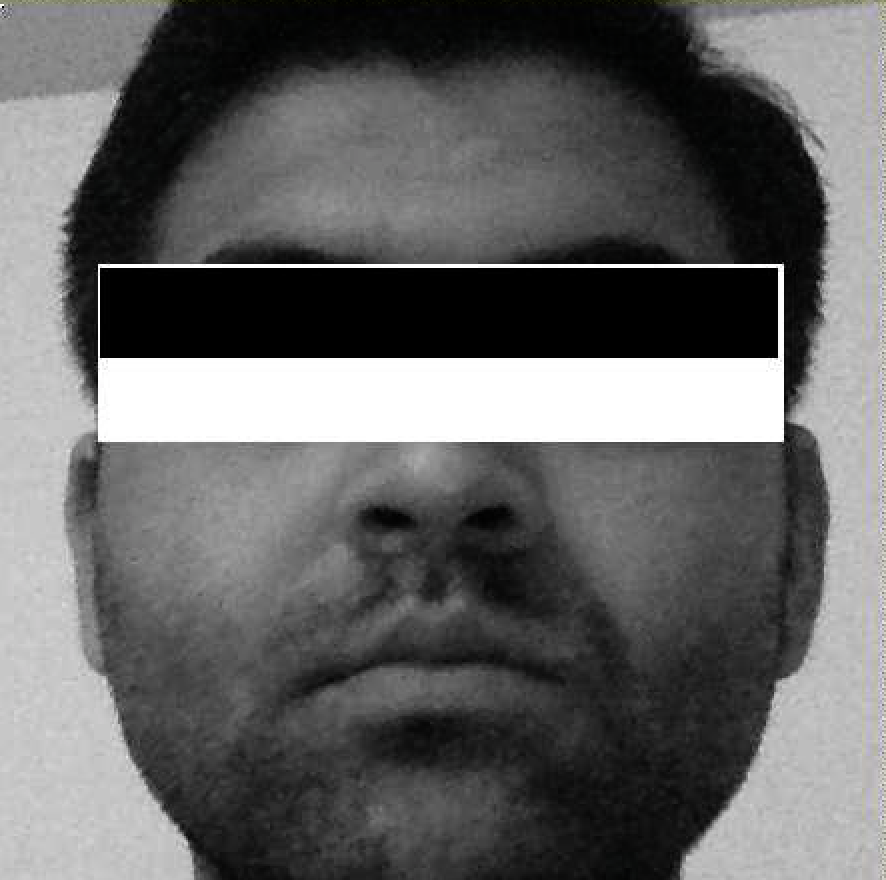
\includegraphics[width=\linewidth]{eyes}
  \end{center}
  \caption{Human eye region haar-feature}
  \label{fig:human_eyes}
\end{figure}


Once we have detected a face, we process frame detected 
as face again using haar-feature based classifier to identify eyes. 

\begin{figure}
  \begin{center}
    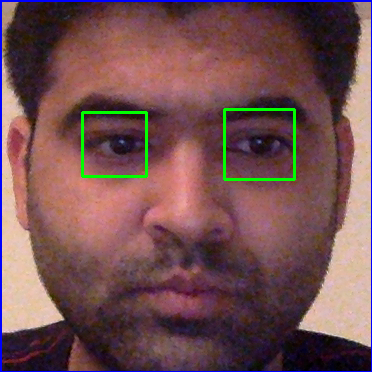
\includegraphics[width=\linewidth]{eyes_detected}
  \end{center}
  \caption{Eye detection using Haar-Cascade When input is identified as face.}
  \label{fig:eyes_detected}
\end{figure}

In our initial runs we encountered difficulties with these cascade classifiers.
This can be seen in  (Figure~\ref{fig:defensive}).
In order to sanitize the inputs passed to our neural network, we added 
additional defensive coding to eliminate false positive detection 
for eyes or faces. We make sure a detected face has eyes 
and location of the eyes are not in the lower half of the detected face

\begin{figure}
  \begin{center}
    \includegraphics[width=\linewidth]{defensive_coding_example}
  \end{center}
  \caption{Failure observed without defensive coding for face and eye
    verification.}
  \label{fig:defensive}
\end{figure}


Once the face itself has been extracted from the video and the eyes
are isolated from the face, then images  of the face and the location
of eyes are fed into a neural network to determine the location of the
gaze.

\subsection{Eye Image Preprocessing}
To aid the neural network, the input data images are preprocessed. We
perform the preprocessing step to aid in locating the pupils withing
the images of the eyes. The pupils of the eyes are distinctive in that
they are, in general, the only large round thing in the eye image. Also,
due to the fact that the iris tends to be of a darker color than the
sclera and therefore should be easily detectable in a grayscale image of the
eye when looking at the gradient of the image. The pupils are
attempted to be located by performing a search for circles in the
Hough space that are of a certain size. The pupils are then added as a
mask to the eye image as a fourth channel in addition to the RGB
images of the eyes. This information is provided as a hint to the
neural network for processing the image. The search for pupils is
limited to circles of a certain size to filter out false matches. The radius of the pupil
in the image is limited to a range between 1/10 to 1/4 relative to the
bounding box size. The range is computed relative to the bounding box
sizes to account for changes in size of the detected eyes in the
captured frames that may account from the user being closer or farther
from the camera. 

\begin{figure}[!h]
  \begin{center}
    \includegraphics[width=\linewidth]{hough-uta-dataset.png}
    \caption{Detection of pupils using Hough space search}
    \label{fig:hough-pupils-uta}
  \end{center}
\end{figure}

\begin{figure}[!h]
  \begin{center}
    \includegraphics[width=\linewidth]{hough-online.png}
    \caption{Detection of pupils during online training and
      inferrence}
    \label{fig:hough-online}
  \end{center}
\end{figure}

We don't only pass the pupil mask
to the neural network because the search in Hough space can result in
either more or less circles in the eye image, or may be offset
slightly from the actual pupils. To counteract this, we provide both
the RGB image of the eye and the mask that we determine locating the
pupils. The detection of the pupil for processing the data set is shown in
Figure~\ref{fig:hough-pupils-uta}. During online training and testing
we also perform a Hough space search for pupils in each image of the
eye. The results for this can be seen in Figure~\ref{fig:hough-online}
which show the capture and processing the pupils. In addition, the
proper left and right eyes needed to be determined, since the list of eyes
detected by the system is unordered. This was done by
ordering the bounding boxes for the two eyes based on the x-location
of the bounding box's upper left corner. The left eye of the user
(looking at the user on the screen) will always have a smaller
x-location coordinate. This ensures that the same eye image and
bounding box is always passed as the same input to the neural network.

\subsection{Convolutional Neural Network}
Our neural network is implemented in the TensorFlow framework. The
network is a multilayer classifier where the inputs are the extracted
images of both the left and the right eyes and the bounding boxes for
both eyes and the bounding box for the face in the original image. The two images of the
eyes are 32x32x4 images where the extracted images of the eyes are
scaled to a set size. This gives us a fixed image size to feed into
the network invariant of the original size of the eyes in the original
video frame. The size of 32x32 should be large enough to provide
enough detail without creating a network that is too large. It is in
line with previous work. 

\begin{figure*}
  \begin{center}
    \includegraphics[width=\textwidth]{gaze-tracking-cnn-arch-final}
  \end{center}
  \caption{Neural Network Architecture}
  \label{fig.cnn-arch}
\end{figure*}

Each eye image is fed into a bank of 16 convolutional filters. This
generates 16 sets of 32x32 filtered results. The filter kernels have
support of 3 pixels in the x- and y-axes. Each pixel output from the
filters is passed through a rectified linear activation function. The
output of the first layer is then again filtered in a convolutional
layer. This layer has a kernel with 5x5 support and generates 64
outputs from the 32 input filter bank output. The outputs from this
layer are again passed through a rectified linear activation function
like before. Following the second convolutional layer, there is a max
pooling layer with a non-overlapping 2x2 filter to reduce the
dimensionality of the output by a factor of two in the x- and y-
directions. This results in a 16x16x64 output. This output is then
filtered once again through a final convolutional layer. This third
layer has a kernel with 3x3 support and results in 64 16x16
outputs. This filter layer is then again passed through a final
max-pooling layer with a non-overlapping 2x2 filter. The final
dimensionality of the output from the convolutional layers is 8x8x64.

The two separate convolutional networks are then combined with the
bounding boxes from the face and eye detection step. The outputs
from the convolutional layers for the left and right eyes are each
flattened into a single 4096x1 vector. These two 4096 vectors and the
bounding boxes are then all concatinated into a single 8204 vector.

Once all of the input features are concatinated together into a single
vector, this is then fed into three fully connected layers of 1024
hidden units. The hidden units also use a rectified linear activation
function. Finally, there is a readout layer at the end with two
nodes. These two nodes are simply a linear combination of the previous
1024 hidden nodes. The output nodes are the x- and y- location of the
users gaze.

The loss function for the network is the simple euclidian squared
error between the predicted x- and y- location of the users gaze and
the ground truth x- and y- location (Equation~\ref{eq:cnn-loss}). As
the network optimizes to minimize the loss, the simple euclidean
distance is then also minimized.

\begin{equation}
  loss = (pred_{x,y} - target_{x,y})^2
  \label{eq:cnn-loss}
\end{equation}

\subsection{Neural Network Datasets}
We used the Point of Gaze Eye-Tracking Dataset from the University
of Texas at Arlington\cite{eyetracking}. This provides a mapping from
a video of eyes to locations in 3D space where the user is
focusing their attention. The dataset consists of data captured from
20 subjects. The dataset for each subject consists of a video of the
user’s eye, transform matrices that relate the user’s eye and the
screen of a display, and the target location on the screen that the
subject is looking at. There are 6 scenarios for each of the 20
users. The transform and the target locations are provided per frame
of the video.

This data set was used to provide initial training for the neural
network. Once we had done initial training of the network on this
dataset, we moved the trained network to running on-line. The goal of
initial training is to speed up the training process for gross
optimization and then be able to fine tune the training using the
actual system. Since the datasets that we used were for specific
transformations between the eyes of the user and the object of the
gaze, the system needed to be trainined to be able to determine the
proper head pose of from the extra inputs from our system and then use
that information to transform the outputs to the correct x- and y-
output.


\section{Experimental Results}


\subsection{Network Training}
During initial gross training, we were able to achive pretty good
results on the UTA dataset\cite{eyetracking}. The system was able to
train both convolutional pipelines quickly over 100 epochs with batch
size of 16 samples. The initial training took a little over an hour on
a MacBook Pro running TensorFlow.

\begin{figure}[!h]
  \begin{center}
    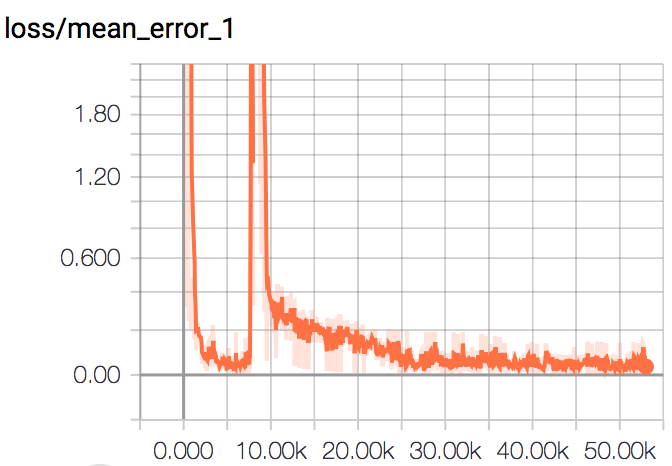
\includegraphics[width=\linewidth]{tb-gross-training-mse-loss.png}
    \caption{Network training loss}
    \label{fig:train-loss}
  \end{center}
\end{figure}

Following the initial training we were getting a mean squared error of
approximagely 0.07 where the range of the gaze of the user was
normalized to the range -0.5 to +0.5. The mean of the squared error
seemed to be skewed by periodic large errors. The intuition behind
this is the the error appears to be very large due to the eye
blinking. The median squared error is much smaller - around 0.03,
again with the range normalized. After initial training, the network
was further refined and valiadated. During this training, the median
training error was refined down to approximately 0.0142, and the
median down the 0.017. With the normalized gaze range, this
corresponds to a median error distance of approximagely 13\% of the
field of view of the viewer.

One of the issues that we faced was the problem of the head pose.
The network needed to still be trained online to calibrate where
the user was looking with the screen relative to the user's head.
Since the system should be able to determine the head pose,
that training needed to be done online so that we can construct the
transformation between the location of the eyes in 3-D space and the
target that the use was looking at. Once that transformation can be
determined then vector that is coming out of the image of the eyes
that represents the direction that the use is looking can be
intersected with the location of the plane of the screen in 3-D
space.

\subsection{System Integration and Testing}
The system integrates the two parts - the face and eye detection, and
the neural network for gaze target determination. To perform our
on-line training, a target was put on the screen for the user to look
at. This target had known x- and y- location on the screen, and this
was used to compute our network loss function. Again, we computed the
euclidean distance between the target on the screen, and the inferred
location that came out of our network. As the target moved around the
screen, this kept getting fed back into the network to compute the
loss and finalize training.

\begin{figure}
  \begin{center}
    \includegraphics[width=\linewidth]{original_object_path}
  \end{center}
  \caption{Path followed by Object on Screen.}
  \label{fig:originalpath}
\end{figure}



\begin{figure}
  \begin{center}
    \includegraphics[width=\linewidth]{predicted_object_path}
  \end{center}
  \caption{Path generated by tracking user’s eye.}
  \label{fig:generatedpath}
\end{figure}


Initially, the target moves across the screen in a couple of
directions for the user to follow. After a few minutes of training,
the system would switch into testing mode where the cursor would
follow the inferred x- and y- positions that the eye was supposed to
be looking at. Our results were that the location generated by our
network would not really move on the screen regardless of where the
user would look. Rather, the point of gaze as determined by the system
would follow the movement of the face on the screen as the user's head
moved around the camera frame.

The first thought was that during training the system was simply
learning the location of the cursor regardless of the input since the
output was mainly changing slowly, and by not a lot of
delta. Therefore, during training, the intuition is that the system
was drifing the entire network around the screen instead of learning
the different locations that the eye could be gazing. To counteract
this, we also implemented an on-line training method to randomly move
the target around the screen in a 3x3 grid of target locations. There
were enough locations around the screen to cover different quadrants
that the user can look, but few enough that the user would be able to
quickly find the target as it moved around the screen. The target
would remain in one area for about 10 frames, and then move to a new
randomly selected location on the screen. Again, this is not really
ideal since we would want to compute the loss for several locations
all at once so that we can accurately compute the gradient to descent
down instead of always chosing to modify the last layer of weights to
move the target into the location on the screen to align with the last
known target location. 

Following this training method, we were still left with the same
issues that we had enountered before. During testing, the determined
gaze location tended to remain stationary on the screen, near the last
location where the training target had been. The issue here we believe
is due to the general latency through the entire closed system. The
latency between the user moving and the time that that movement can be
captured by the system seems to be on the order of about a
second. At around 10 fps throughput of the system, this means that
there is about 10 frames of delay in the system. What we believe is
happening is that from when the target is displayed on the screen to
when the determination is made as to the location of the user's gaze
is about 10 frames. This means that when the loss is computed during
training, comparing the target location and the inferred gaze
determination the comparison and loss computation is done on two
points in time that are not synchronized. In this case, the target and
the predicted gaze location are completely uncorrelated, and no proper
training can take place.

The fact that the predicted gaze target location tended to follow the
location of the face and eyes of the user indicates that the bounding
boxes for the user features are having an overriding influence on the
weights of the system in the connected layer, with the movement of the
pupils inside the bounding boxes being marginalized.

\section{Future Work and Directions}
Our results seem promising, but there are some issues that will need
to be resolved. First, we believe that the lag through the system
should be addressed. This would aid in any training that we may need
to perform. The closer we can get between the display of the actual
target on the screen and the determination of where the user is
looking would help in training such that the target and the prediction
are correlated in time to have consistant inputs to train the
network.

Second, in order to do more training off-line and not rely on on-line
training, to assemble a full synchronized data set offline where the
target locations and the captured images from the camera are in sync
with each other so that they can be used to batch train the network
off-line. This would speed up the training time (not just of where the
eyes are looking with respect to the eye socket, but also for
determining the head pose off line with respect to the camera). The
data set could then be shuffled, like the UTA dataset was suffled for
training, and keep the entire system from just drifting to the last
location of the target.

Third, we should split the convolutional network into it's different
parts. The thinking is that we can construct three networks. One for
mapping the eye image to a relative angle of view from the eye, one
for each of the left and right eyes. Then these outputs can be fed
into a much smaller fully connected network that would perform the
head pose transformation to the final output predicted gaze target on
the screen. With this, we can train the two convolutional networks on
the images of the eyes, and then we can perform and head pose training
separately on-line in the system. Since the networks are separate, we
can then not train the convolutional networks, but just the final
transformation network. This would prevent the on-line training from
interfearing with the learned parameters for the convolutional network.

Finall, We believe limited frame rate of the built in laptop and tablet front facing cameras was another 
factor in our experiment. The latest commercial solution by Tobii like "Tobii X3-120", has a sampling 
rate of 120 frames per second, which is 10x of what our system is able to process in its current state. 
We also believe implementing such solution on latest handheld devices like iPhoneX, which 
come pre-equiped with an infrared sensor(dot projector and receiver), is more viable in near future. 
If more devices came pre-equiped with such sensors, then gaze tracking will be just a software application away. 

 

We have shared our code publicly on github @ https://github.com/tomkarpati/cs231a-gaze-tracking.git 
and we invite all people interested in this cause to take a look at our implementation, and help us enhance it to perfection.






{\small
\bibliographystyle{ieee}
\bibliography{egbib}
\begin{thebibliography}{1}
\bibitem{calvo}
  Calvo A. et al.. Eye Tracking Impact on Quality-of-Life of ALS
  Patients. In: Miesenberger K., Klaus J., Zagler W., Karshmer
  A. (eds) \underline{Computers Helping People with Special Needs. ICCHP
    2008}. \underline{Lecture Notes in Computer Science}, vol 5105. Springer,
  Berlin, Heidelberg, 2008
\bibitem{eyetracking}
  http://heracleia.uta.edu/~mcmurrough/eyetracking/
\bibitem{krafka}
  Krafka, Kyle, et al. Eye tracking for everyone.
  \textit{IEEE Conference on Computer Vision and Pattern Recognition
    (CVPR)}, 2016
\bibitem{mcmurrough}
  McMurrough, Christopher D., et al. "A dataset for point of gaze
  detection using head poses and eye images."
  \textit{Journal on Multimodal User Interfaces 7.3} (2013): 207-215.
\bibitem{weidenbacher}
  Weidenbacher, U.; Layher, G.; Strauss, P.-M.; Neumann, H.: "A
  comprehensive head pose and gaze database",
  \textit{IET Conference Proceedings}, 2007
\bibitem{baluja}
  Baluja, Shumeet, and Dean Pomerleau. "Non-intrusive gaze tracking
  using artificial neural networks." \textit{Advances in Neural
    Information Processing Systems}. 1994.
\bibitem{cazzato}
  Cazzato, D., Dominio, F., Manduchi, R., and Castro, S. M.,
  “Real-time Gaze Estimation Via Pupil Center Tracking”,
  Paladyn. \textit{Journal of Behavioral Robotics}, In Press.
\bibitem{li}
  Li, Tianxing, et al. "Ultra-Low Power Gaze Tracking for Virtual
  Reality." \textit{Proceedings of the 23rd Annual International
    Conference on Mobile Computing and Networking}. ACM, 2017.
\bibitem{lecun_1}
  LeCun, Yann, et al. "Handwritten digit recognition with a
  back-propagation network." \textit{Advances in neural information
    processing systems}. 1990.
\bibitem{lecun_2}
  Le Cun, Yann, et al. "Handwritten zip code recognition with
  multilayer networks." \textit{Pattern Recognition,
    1990. Proceedings., 10th International Conference
    on}. Vol. 2. IEEE, 1990.
\bibitem{eyetrackerlist}
  http://www.eyetracking.com/Hardware/Eye-Tracker-List
\bibitem{tobii_1}
  https://www.tobiidynavox.com/en-US/products/devices/
\bibitem{tobii_2}
  https://www.tobii.com/group/about/this-is-eye-tracking/

\end{thebibliography}
}

\end{document}
